\documentclass[journal, table]{IEEEtran}
\usepackage[english, spanish]{babel}
\usepackage[sorting=none]{biblatex}
\bibliography{ref.bib}
\usepackage{amsmath, amsfonts, amsthm}
\usepackage{hyperref, url}
\hyphenation{op-tical net-works semi-conduc-tor}
\usepackage{graphicx}
\usepackage{float}
\usepackage{fancyhdr, last page}
\usepackage{siunitx}
\usepackage{anyfontsize}
\usepackage{csquotes}
\usepackage{svg}
\usepackage{tabularx, ragged2e, booktabs}
\usepackage{xcolor}
\usepackage{multirow}
\usepackage{adjustbox}
\usepackage[affil-sl]{authblk}
\usepackage{tikz}
\usepackage[spanish]{cleveref}
\usepackage{circuitikz}
\usetikzlibrary{patterns}
\usepackage{scalerel}
\usepackage{pict2e}
\usepackage{tkz-euclide}
\usetikzlibrary{calc}
\usetikzlibrary{arrows.meta}
\usetikzlibrary{shadows}
\usetikzlibrary{external}
\usetikzlibrary{decorations.pathmorphing}
\usetikzlibrary{shapes.geometric}
\usetikzlibrary{arrows,shapes.gates.logic.US,shapes.gates.logic.IEC,calc}
\usepackage{pgfplots}
\pgfplotsset{compat=newest}
\usepgfplotslibrary{statistics}
\usepgfplotslibrary{fillbetween}

\AtBeginDocument{\decimalpoint}

\graphicspath{images}
\hypersetup{
    colorlinks=true,
    linkcolor=black,
    urlcolor=blue,
    pdftitle={ALU-JLAB}
}
\urlstyle{same}
\sisetup{separate-uncertainty}

\begin{document}
\tikzstyle{branch}=[fill,shape=circle,minimum size=3pt, inner sep=0pt]

\title{\textbf{Unidad Aritmético-lógica} \\ \small{ALU}}

\author[*]{Julian Avila
    \thanks{Julian Avila: 20212107030}}
\author[*]{Laura Herrera
    \thanks{Laura Herrera: 20212107011}}
\author[*]{Bryan Martínez
    \thanks{Bryan Martínez: 20212107008}}
\author[*]{Juan Acuña
    \thanks{Juan Acuña: 20212107034}}

\affil[*]{Proyecto Curricular de Física\\ Universidad Distrital Francisco José de Caldas}

\date{\today}

\markboth{}
{Shell \MakeLowercase{\textit{et al.}}: Bare Demo of IEEEtran.cls for IEEE Journals}

\maketitle

\section{Objetivos}
\begin{itemize}
    \item Diseñar una unidad aritmético-lógica para dos números de 4-bits mediante lógica combinacional.
    \item Visualizar usando LEDs el resultado de la correspondiente operación de la ALU.
\end{itemize}

\section{Diseño y solución del problema}
Se plantea realizar una unidad aritmético-lógica (ALU) para dos números de 4 bits.
Para la parte lógica, el circuito realizará las siguientes operaciones:

\begin{gather}
    A \land B \\
    A \lor B \\
    A \oplus B \\
    \bar{A}
\end{gather}

En la parte aritmética se realizan las siguientes operaciones:
\begin{gather}
    A+B \\
    A-B \\
    A+1 \\
    A-1
\end{gather}

Para poder generar las diferentes opciones que tiene la ALU se hizo uso de MUXs,
de esta forma el usuario puede escoger qué operación desea visualizar entre los números ingresados.\cite{wakerly-1989}

Para la parte aritmética, se utiliza un IMUX y dos MUX, el IMUX y uno de las MUX
tienen la función de escoger si $A$ se va a operar con $B$ o con 1.
El segundo MUX tiene la función de escoger si se visualiza suma o resta aritmética de los números escogidos.

Para la parte lógica se utilizan tres MUX, los cuales se encargan de filtrar que
operación se va a visualizar ya sea $A \land B$, $A \lor B$, $\bar{A}$ o $A \oplus B$.
En el caso de las operaciones lógicas, se realizan mediante comparación bit a bit de ambos inputs.

Finalmente, para el resultado que se visualice en 5 LEDs, se utiliza un MUX
el cual permite eligir entre el resultado de la operación aritmética o la lógica.

\section{Diagrama de compuertas Lógicas y Circuito}
\subsection{Sub-Unidad Aritmética}
\begin{figure}[h]
    \centering
    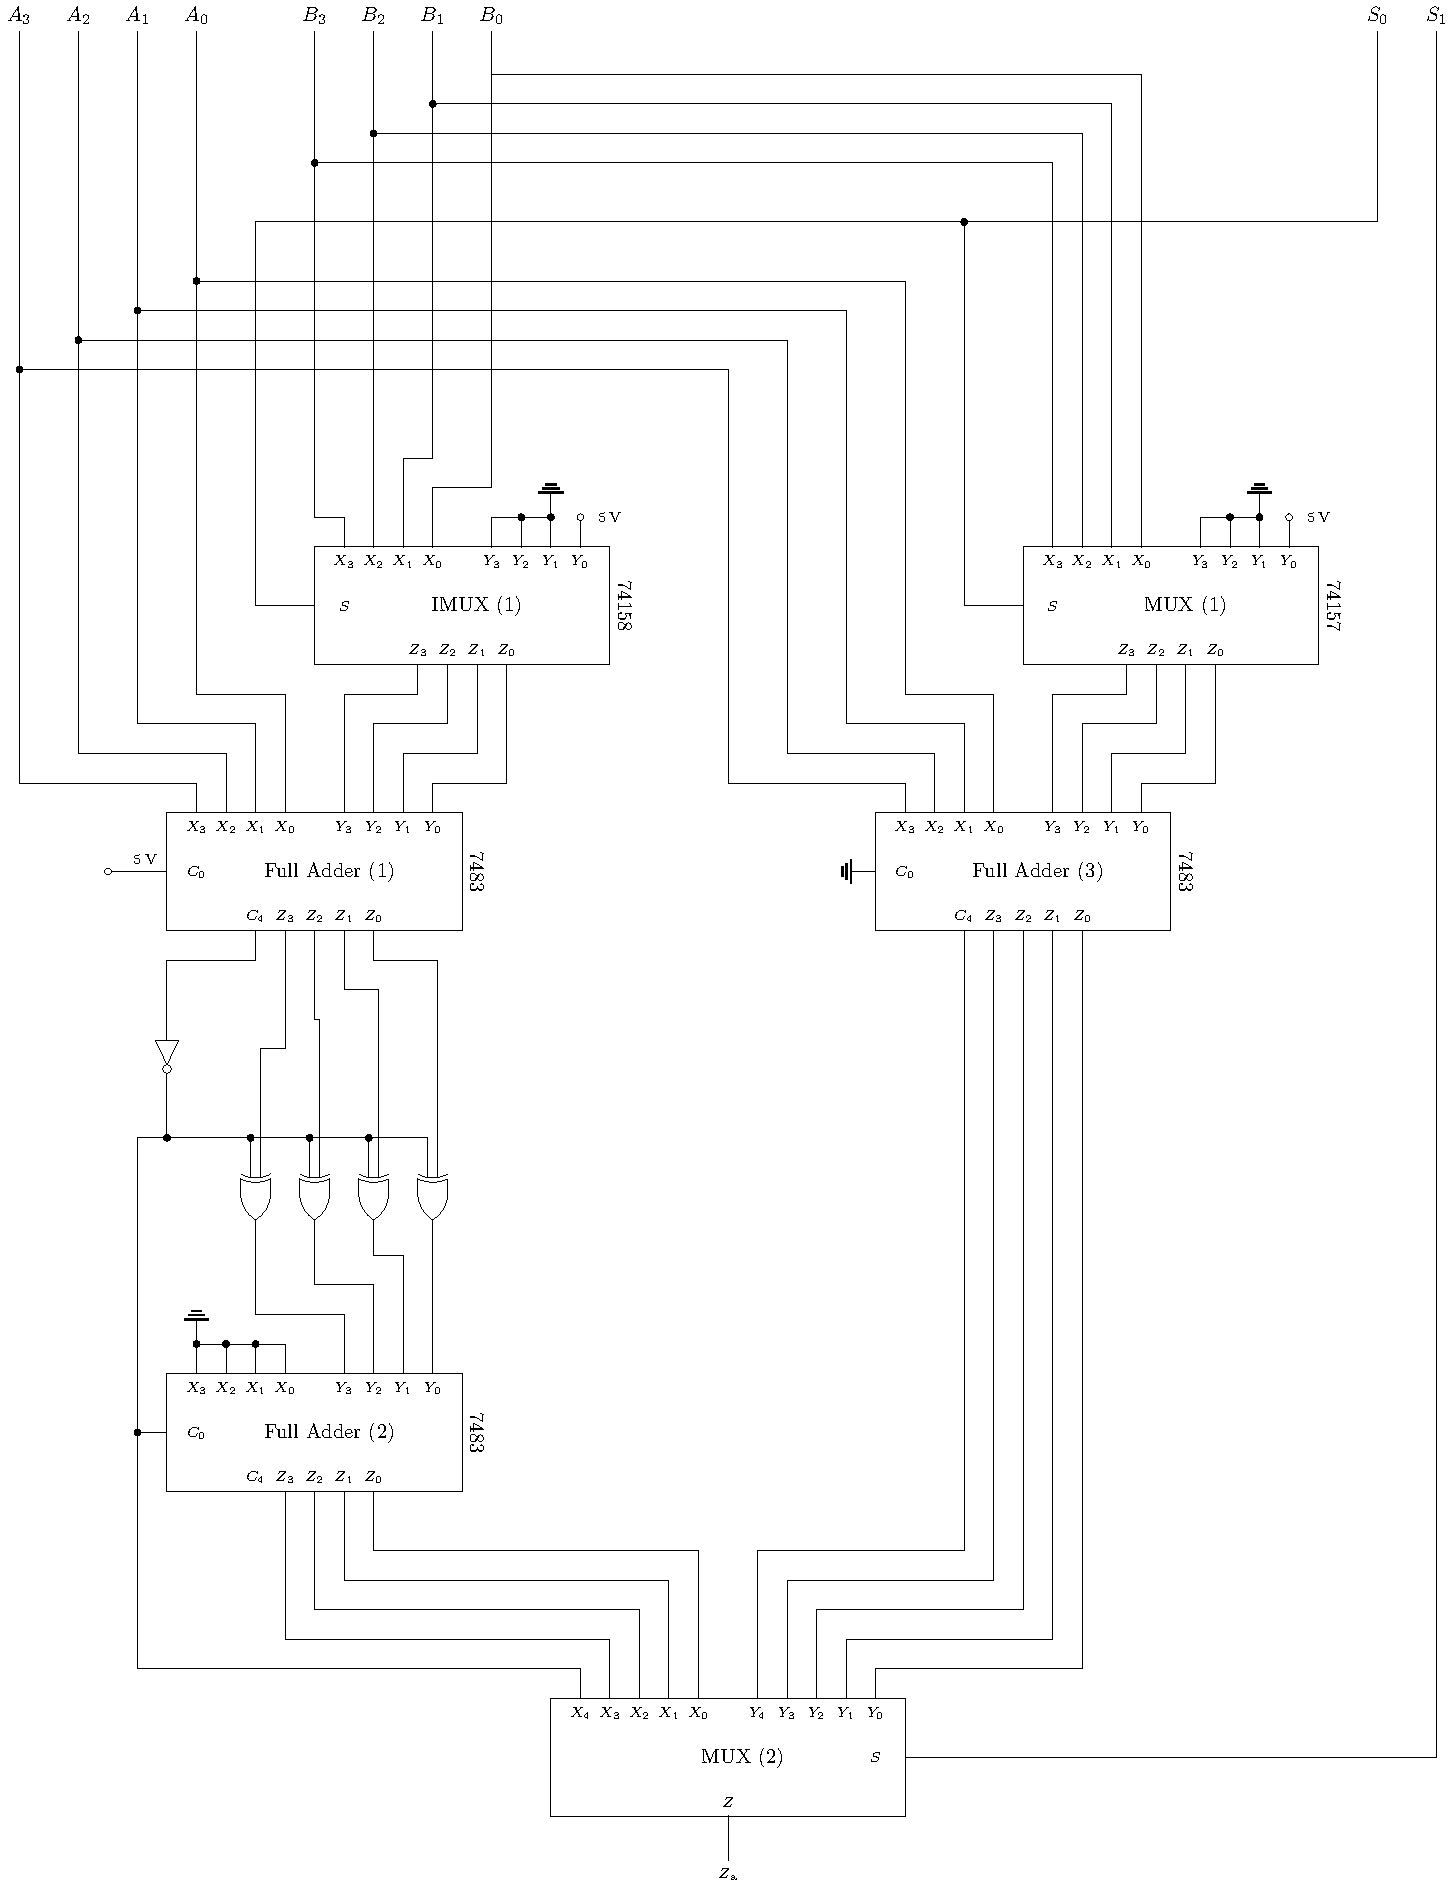
\includegraphics[width=\linewidth]{./Images/arithmetische.pdf}
    \caption{Diagrama de la parte aritmética.}
    \label{fig:arithmetic-diagram}
\end{figure}

Como primer sub-unidad se tiene la parte aritmética, en esta se realizan las operaciones
entre dos números de 4 bits que ingresan como input. La resta entre $A$ y $B$
o el decrementar $A$ se realiza con la suma del complemento a 2 del sustraendo,
por ello se utilizan 2 Full Adder, el primero para el complemento a dos y la suma,
y el segundo permite corregir el resultado si el valor real es menor a 0,
complementando a 2 el resultado del primer Full Adder.
El resultado se presenta en 5 LEDs, donde el de mayor significancia funciona como indicador de signo.

Para la suma, dependiendo si se le desea sumar $B$ o $1$ a $A$, se utiliza un Full Adder,
el resultado es un numero de 5-bits mayor a 0, por ello el bit de mayor significancia
presenta un peso de $2^4$.

\subsection{Sub-unidad Logica}
\begin{figure}[h]
    \centering
    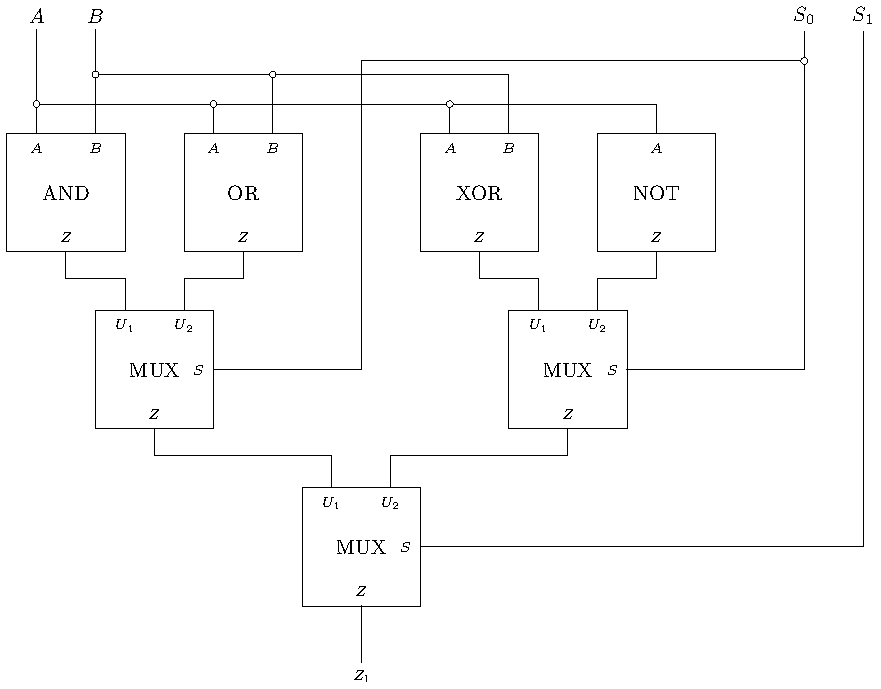
\includegraphics[width=\linewidth]{./Images/logik.pdf}
    \caption{Diagrama de la parte lógica.}
    \label{fig:logic-diagram}
\end{figure}

La segunda sub-unidad es la parte lógica, se toman las entradas de 4-bits y son
comparadas por cada operación bit a bit. La única operación unitaria es $\bar{A}$.

\subsection{Unidad Aritmético-lógica}

La unidad completa toma las salidas de las dos sub-unidades y filtra el resultado
deseado según la señal de entrada $S_2$ para ser mostrado por 5 LEDs.
La siguiente tabla muestra el resultado mostrado según el estado de las señales
de control $S_0, S_1, S_2$:

\begin{table}[htbp!]
    \centering
    \rowcolors{2}{white}{gray!25}
    \begin{tabular}{c|c|c||c}
    \toprule
        $S_2$ & $S_1$ & $S_0$ & $Z$ \\
        \midrule
        0 & 0 & 0 & $A - B$ \\
        0 & 0 & 1 & $A - 1$ \\
        0 & 1 & 0 & $A + B$ \\
        0 & 1 & 1 & $A + 1$ \\
        1 & 0 & 0 & $A \land B$ \\
        1 & 0 & 1 & $A \lor B$ \\
        1 & 1 & 0 & $A \oplus B$ \\
        1 & 1 & 1 & $\Bar{A}$ \\
        \bottomrule
    \end{tabular}
    \caption{Tabla de salidas según las señales de control.}
    \label{tab:Zvalue}
\end{table}

\begin{figure}[h]
    \centering
    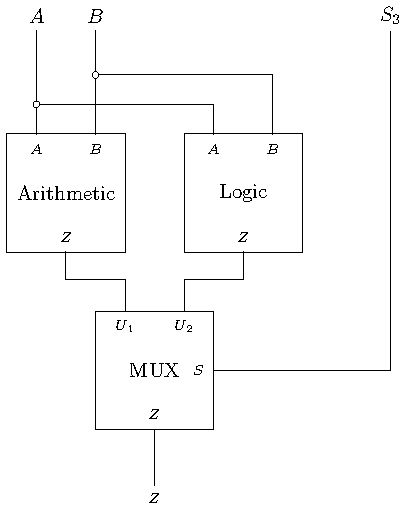
\includegraphics[width=\linewidth]{./Images/alu.pdf}
    \caption{Diagrama de la ALU.}
    \label{fig:alu-diagram}
\end{figure}

\subsection{Fotos del circuito}
\begin{figure}[H]
    \centering
    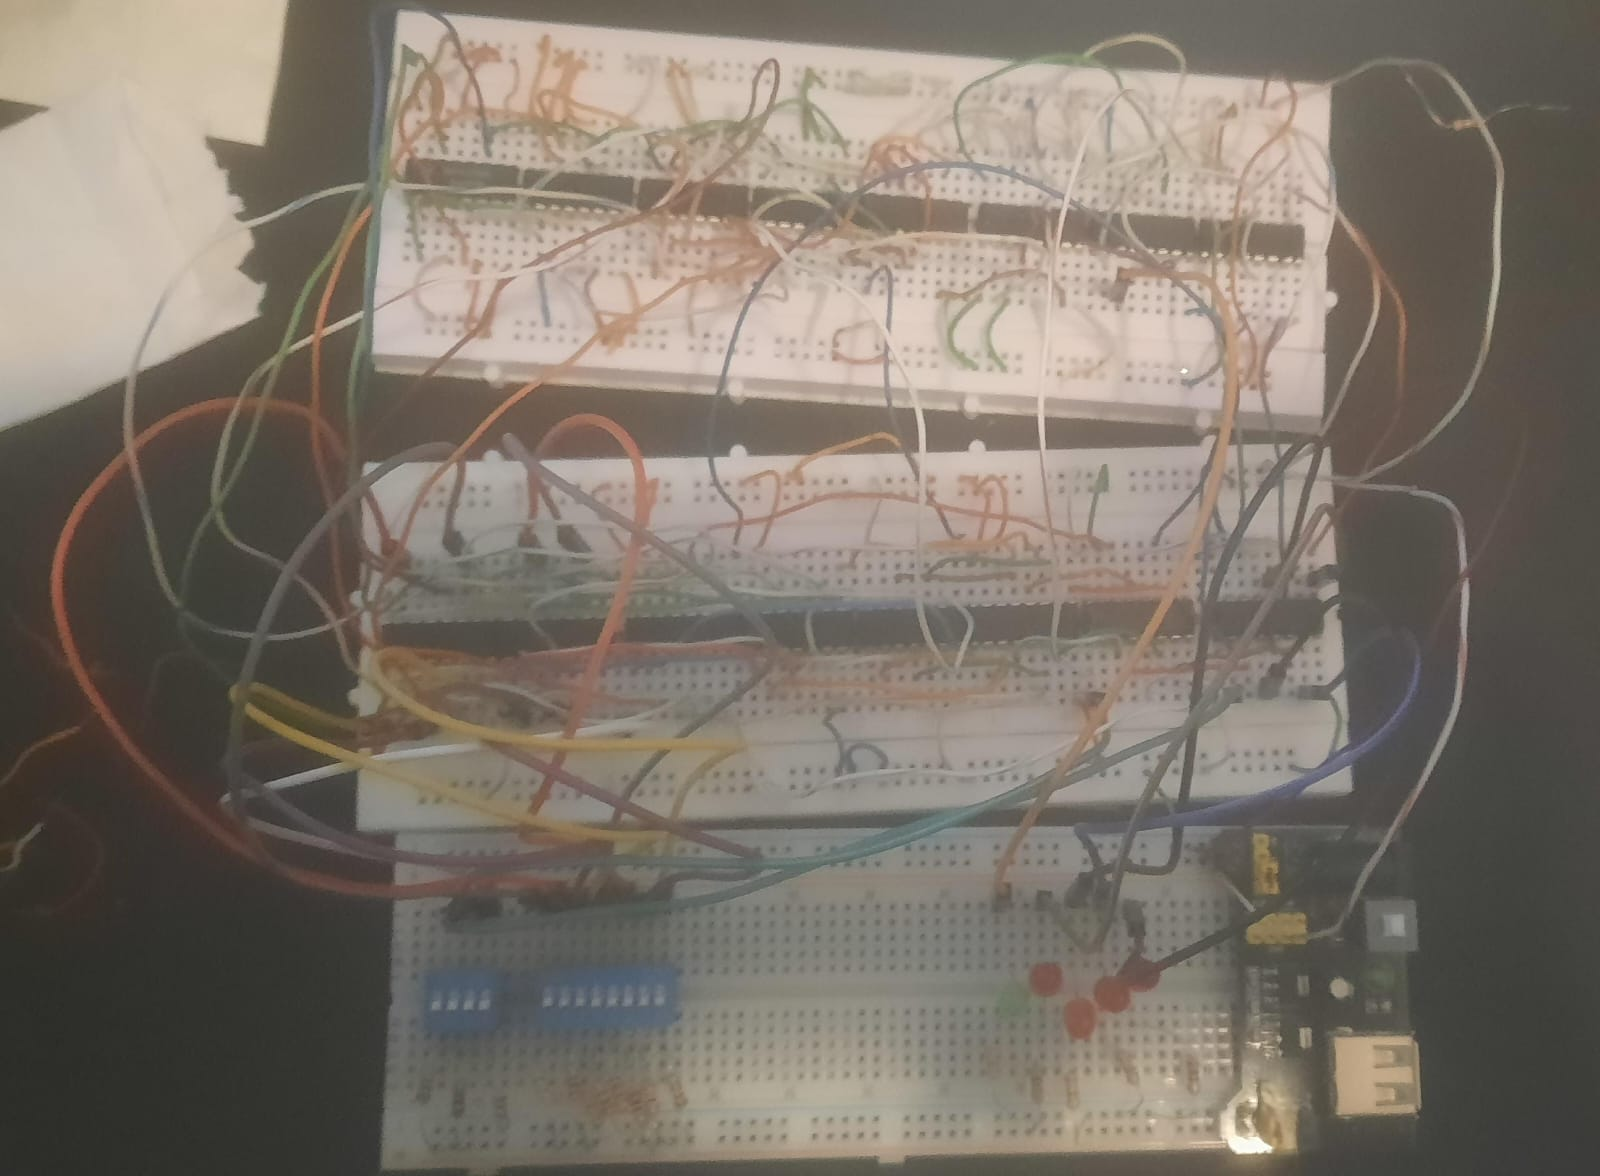
\includegraphics[width=\linewidth]{./Images/WhatsApp Image 2024-05-11 at 18.46.47.jpeg}
    \caption{Foto del montaje del circuito.}
    \label{fig:photo}
\end{figure}

\section{Conclusiones}
Se diseño una unidad aritmético-lógica para dos números de 4-bits a partir del
uso de compuertas lógicas, y lógica combinacional utilizando un total de 6
multiplexores, un multiplexor inversor, 3 Full Adders, 5 compuertas NOT,
4 compuertas AND, 4 compuertas OR, 8 compuertas XOR.

\printbibliography
\nocite{*}

\end{document}
